%!TEX encoding = UTF-8 Unicode
% !TeX spellcheck = en_GB

%%%%%%%%%%%%%%%%%%%%%%%%%%%%%%%%%%%%%%
\chapter{ Overview of Higgs pair production at colliders }\label{chap:overviewDiHiggs}
%%%%%%%%%%%%%%%%%%%%%%%%%%%%%%%%%%%%%%
The dominant process for Higgs pair production at the LHC~(and hadron colliders in general) is the gluon gluon fusion~(ggF) via a heavy quark loop~$Q$, mainly the top and beauty quark, with the latter contributing only to about~$1\%$, see figure~\ref{fig_ggf_sm}.
%
\begin{figure}[!htpb]
	\centering
	\includegraphics[width = 0.35\textwidth]{./figures/ggfbox}
	\hspace{0.3 cm}
	\includegraphics[width = 0.4\textwidth]{./figures/ggftri}
	\caption{Feynman diagrams for the ggF process of Higgs pair production in the SM.} % verify the notation
	\label{fig_ggf_sm}
\end{figure}
%
This process is well-studied at leading order~(LO) analytically \cite{EBOLI1987269,GLOVER1988282,DICUS1988457,Plehn:1996wb}. The next-to-leading  QCD order~(NLO)   was initially computed using infinite top mass limit~($m_t \to \infty$) using the Higgs effective field theory~(HEFT) and implemented in the programme \texttt{Hpair}~\cite{Dawson:1998py}. However, this approximation is not suitable for obtaining distributions, and using numerical methods~\cite{Borowka:2016ypz,Borowka:2016ehy,Baglio:2018lrj} the full NLO results were obtained. In ~\cite{Heinrich:2019bkc}, parton shower effects were included in the NLO calculations, allowing the use of the NLO in event generators such as \textsc{Pythia} and \textsc{Powheg}. Analytical calculations for the NLO corrections using small Higgs transverse momentum~$p_{T,h} \to 0$ yielded a good estimation for the numerical result~\cite{Bonciani:2018omm}. The use of Pad\'e approximation obtained also analytical results for the NLO result and a description for the three-loop~(NNLO) form factors~\cite{Davies:2019nhm}. The NNLO cross section with top mass effects has been computed numerically in~\cite{Grazzini:2018bsd}.
%
\par
%
{}
In this work, we have calculated the  $ \sqrt{s} = 14$ \text{TeV}  LO ggF inclusive cross-section and distributions with modified light Yukawa couplings by including the light quark loops and the coupling $hh q \bar q$ described in the last diagram in figure~\ref{fig_ggf_diag} .
\begin{figure}[!htpb]
	\centering
	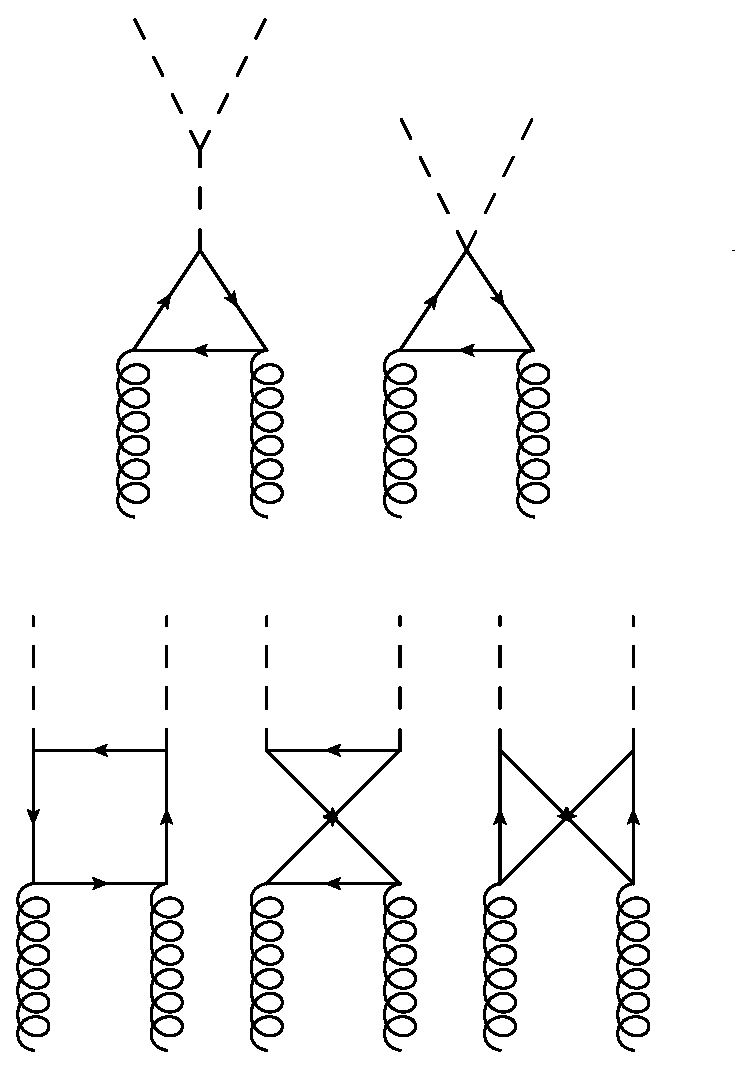
\includegraphics[width = 0.4\textwidth, angle =-90]{./figures/gg_hh_lo}
	\caption{The one-loop diagrams calculated in the ggF with modified Yukawa couplings}
	\label{fig_ggf_diag}
\end{figure}
The calculation was carried out using a FORTRAN code utilising the \texttt{VEGAS} integration algorithm, and NNPDF30 parton distribution functions~(PDF's)\cite{Ball:2017nwa} implemented via \texttt{LHAPADF-6} package\cite{Buckley:2014ana}. For the loop integrals~(see Appendix), we have used the \textsc{Collier} library~\cite{Denner:2014gla} for regularisation of the IR divergent light quark loops, that were assumed massless. A $K$-factor, for the NNLO correction were used according to the Higgs cross section working group recommended values~\cite{Dittmaier:2012vm,deFlorian:2016spz}:
\begin{equation}
	K = \frac{\sigma_{NNLO}}{\sigma_{LO}}, \;\;\;\;\; K_{14 \mathrm{TeV}} \approx 1.71.
\end{equation}
Since the cross-section is not expected to change a lot by changing the light Yukawa couplings, we use the same NNLO K-factor for all values of the scalings.
The renormalisation~$\mu_R$ and factorisation~$ \mu_F$ scales of the $\alpha_s$ and PDF running are set to $\mu_0 =0.5\, M_{hh}$, and $\alpha_s(M_Z) = 0.118$. In our calculations, we did not consider the quark mass running, as the later will be accounted for in the K-factor.
\subsubsection{Theoretical systematic uncertainties}
There are three main sources of theoretical \textit{systematic} uncertainties:
\begin{enumerate}
	\item Scale uncertainty: coming form the arbitrariness of scales choice.
	\item PDF uncertainties : coming form the uncertainty in the PDF fitting and model.
	\item $\alpha_s$ running uncertainty: originating from the initial value (i.e. $\alpha_s(M_Z) $).
\end{enumerate}
In order compute these uncertainties, we follow the recommendations of the Higgs cross-section working group for the value and uncertainty of $\alpha_s$
\begin{equation}
	\alpha_s(M_Z) = 0.1180 \pm 0.0015,
\end{equation}
and the methods described in ~\cite{Martin:2009bu, Demartin:2010er}. for PDF and $\alpha_s$ uncertainties.
% should I put the formula ?
In order to calculate the scale uncertainties, the cross-section was computed with different $ \mu_R$ and $\mu_F$ values ranging between:
\begin{equation}
	\frac{M_{hh}}{4} \leq \mu_R/\mu_F  \leq \,M_{hh}
\end{equation}
The scale uncertainty for the LO total cross-section was found to be $+20\%, -16 \%$. Moreover, the PDF$+\alpha_s$ uncertainty was $\pm 6.8\%$.
\subsubsection{results}
The total cross sections with their uncertainties is shown in table~\ref{ggf_xsres}.
%
\begin{table}
	\centering
	\begin{tabular}{ccccc}
		\toprule
		& $ \sigma$	[fb] & Scale [fb] & PDF$+\alpha_s$ [fb]& Total [fb] \\
		\midrule
		SM HEFT  (LO)      &  $ 18.10$    &   $-$      & $-$   &  $-$ \\
		SM   running mass (LO)  &  $ 16.96$    &   $ -$   & $-$   &  $-$ \\
		SM    (LO)  &  $ 21.45$    &   $ \,^{+4.29}_{-3.43}$   & $\pm 1.46$   &  $ \,^{+4.53}_{-3.73}$ \\
		SM   (NLO)~\cite{Baglio:2012np}  &  $ 33.89$   &   $ \,^{+6.17}_{-4.98}$   & $ \,^{+2.37}_{-2.01}$   &  $ \,^{+6.61}_{-5.37}$ \\
		SM   (NNLO)~\cite{Grazzini:2018bsd}  &  $36.69$    &    $ \,^{+0.77}_{-1.83}$   & $\pm 1.10$    ($g_{hq \bar q} = g_{h b \bar b}^{SM}$) &  $ \,^{+1.66}_{-6.43}$ {\tiny(incl. $m_t$ uncertainty)} \\
		($g_{hq \bar q} = g_{h b \bar b}^{SM}$)  (ggF-LO)  &  $ 21.84$    &  $ \,^{+4.38}_{-3.51}$   & $\pm 1.49$   &  $ \,^{+4.62}_{-3.81}$ \\
		\bottomrule
	\end{tabular}
	\label{ggf_xsres}
	\caption{Gluon fusion~(ggF) Higgs pair production cross-section with theoretical systematic uncertainties, for infinite top mass limit (SM HEFT), running mass, LO, NLO and NNLO QCD corrections. The NLO and NNLO results are taken from the references cited in the table. We also state the benchmark point ($g_{hq \bar q} = g_{h b \bar b}^{SM}$)  cross section result (all the light Yukawa couplings are scaled to the SM beauty Yukawa )}
\end{table}